\section{Empirical Results}

\subsection{Overview of the output set}

The final pipeline produces a complete set of empirical artifacts: out-of-sample metrics, model rankings, Diebold--Mariano comparisons, investor-signal statistics, prediction files, and thesis-ready figures. This matters because the contribution of the thesis is not limited to one isolated table. The project generates a consistent collection of results that can be inspected from several complementary angles: average forecast accuracy, statistical significance of differences, regime-specific diagnostics, and practical stress warnings.

At the broadest level, the results support the claim that the dependency process is forecastable. However, they also show that the forecasting problem is dominated by target persistence. This means that the thesis produces a scientifically meaningful result, but not a simplistic story in which the most complex model necessarily wins.

\subsection{Average dependency-forecasting performance}

Table~\ref{tab:model_ranking_summary} summarizes the average out-of-sample performance of the main models across all dependency experiments. The ranking is based primarily on RMSE.

\begin{table}[H]
    \centering
    \caption{Average forecasting performance across dependency experiments.}
    \label{tab:model_ranking_summary}
    \begin{tabular}{lrrr}
        \toprule
        Model & Average RMSE & Average MAE & Average $R^2$ \\
        \midrule
        AR1 & 0.0667 & 0.0405 & 0.9421 \\
        Naive\_Last & 0.0674 & 0.0396 & 0.9409 \\
        Ridge & 0.0916 & 0.0637 & 0.8914 \\
        ElasticNet & 0.0923 & 0.0644 & 0.8898 \\
        RF & 0.1013 & 0.0711 & 0.8687 \\
        GBM & 0.1038 & 0.0734 & 0.8622 \\
        XGB\_GPU & 0.1057 & 0.0758 & 0.8566 \\
        DCC\_GARCH & 0.2345 & 0.1848 & 0.2788 \\
        \bottomrule
    \end{tabular}
\end{table}

Several points are immediately visible. First, the best average model is not the most complex one but the AR1 baseline. Second, the naive persistence model is almost indistinguishable from AR1 in average RMSE. Third, regularized linear machine-learning models occupy a middle position and outperform tree ensembles on average. Fourth, DCC-GARCH is clearly weaker than all major alternatives in this dataset and evaluation setting.

The interpretation is straightforward but important. The dependency target is strongly persistent, and that persistence carries most of the predictive signal. This is why the simplest autoregressive structures dominate the ranking. A more complex model cannot gain much unless it extracts information beyond what is already contained in the lagged dependency itself.

\subsection{Representative forecast example}

Figure~\ref{fig:sp500_forecast} shows a representative out-of-sample forecast panel for the Bitcoin--S\&P 500 pair using the 30-day rolling window. This pair is substantively important because it links the cryptocurrency market to a broad benchmark of conventional equity risk.

\begin{figure}[H]
    \centering
    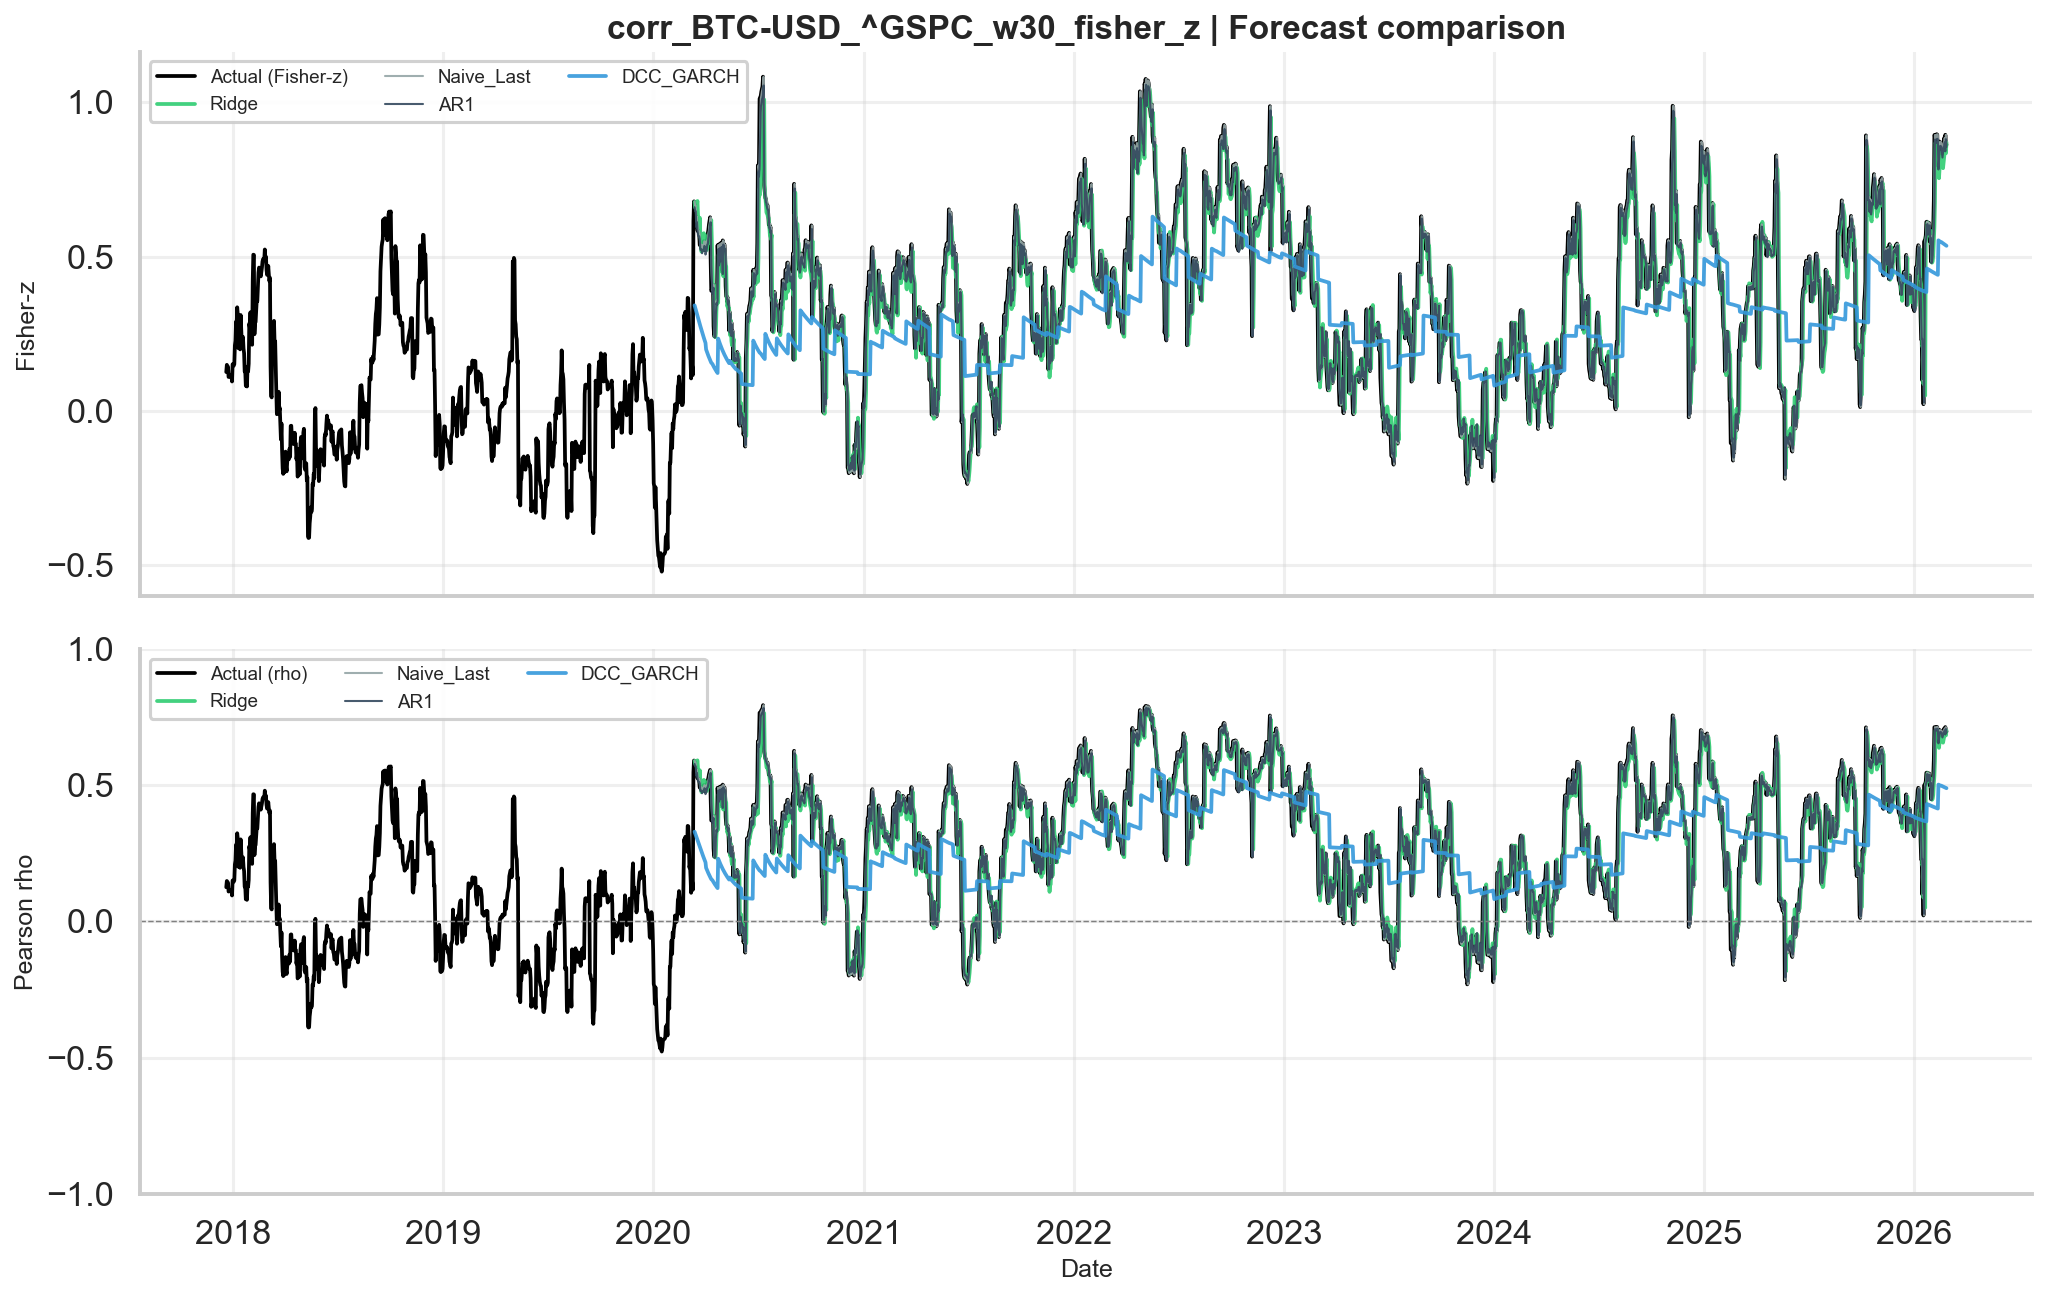
\includegraphics[width=0.95\textwidth]{../outputs/figures/thesis_forecast_corr_BTC-USD_^GSPC_w30_fisher_z.png}
    \caption{Observed and predicted dependency for the Bitcoin--S\&P 500 pair at the 30-day window.}
    \label{fig:sp500_forecast}
\end{figure}

The figure illustrates several characteristic features of the forecasting problem. First, the target moves in a relatively smooth manner, consistent with the use of rolling-correlation construction. Second, the strongest models track broad directional changes reasonably well. Third, local regime shifts remain difficult, particularly when the dependency process changes rapidly. This is exactly the type of environment in which a DCC benchmark may lag and where flexible machine-learning methods can sometimes provide a relative improvement even if they do not beat persistence baselines on average.

\subsection{Forecasting performance by asset class}

The average model ranking hides useful cross-asset variation. The BTC--ETH dependency tends to be the easiest to forecast because the two assets belong to the same broader market complex and often co-move strongly. This is reflected in very high out-of-sample $R^2$ values, especially for longer rolling windows, where the dependency target becomes even smoother.

Gold- and silver-related dependencies occupy an intermediate position. The rolling correlation between Bitcoin and gold or silver does exhibit structure, but it is less stable than the cross-crypto relation and may alternate between low, weakly positive, and weakly negative regimes. Even so, the experiments show that these targets remain forecastable and that persistence-based models are particularly strong.

The equity-index pairs, Bitcoin--S\&P 500 and Bitcoin--NASDAQ, are arguably the most relevant from a practical portfolio perspective. These relations matter because they connect crypto behavior with broad risk appetite. The results show that these dependencies are forecastable, but they also reveal substantial regime sensitivity. In some periods, the relation looks like a shared risk-on factor; in other periods, it weakens or reconfigures.

The dollar-index proxy pair has the weakest practical investor interpretation but remains analytically useful. It captures whether Bitcoin's dependency with a macro-defensive instrument is sufficiently structured to carry forecastable information. The answer is mixed but still informative.

\subsection{Why simple models dominate}

A central empirical finding of the thesis is that simple models dominate average performance. This does not invalidate the machine-learning approach. Instead, it clarifies the nature of the target. Because rolling dependency is a persistent, smoothed object, the one-step-ahead forecasting task is close to a persistence problem. Any complex model that attempts to outperform this baseline must learn subtle deviations from persistence rather than the bulk of the target dynamics.

This observation is reinforced by the feature-importance diagnostics from the Random Forest analysis. The lagged dependency term overwhelmingly dominates the ranking, while additional features such as local return volatility or return spreads contribute only marginally. In practical terms, the thesis shows that the problem is forecastable primarily because the target remembers its recent past.

\subsection{Comparison with DCC-GARCH}

Even though simple baselines dominate overall performance, machine learning remains useful in benchmark comparison. The DCC-GARCH model is a natural econometric reference point, but in this empirical setting it is not competitive on average. Figure~\ref{fig:dm_heatmap} presents a heatmap summary of the Diebold--Mariano comparison between a strong machine-learning candidate and the DCC benchmark.

\begin{figure}[H]
    \centering
    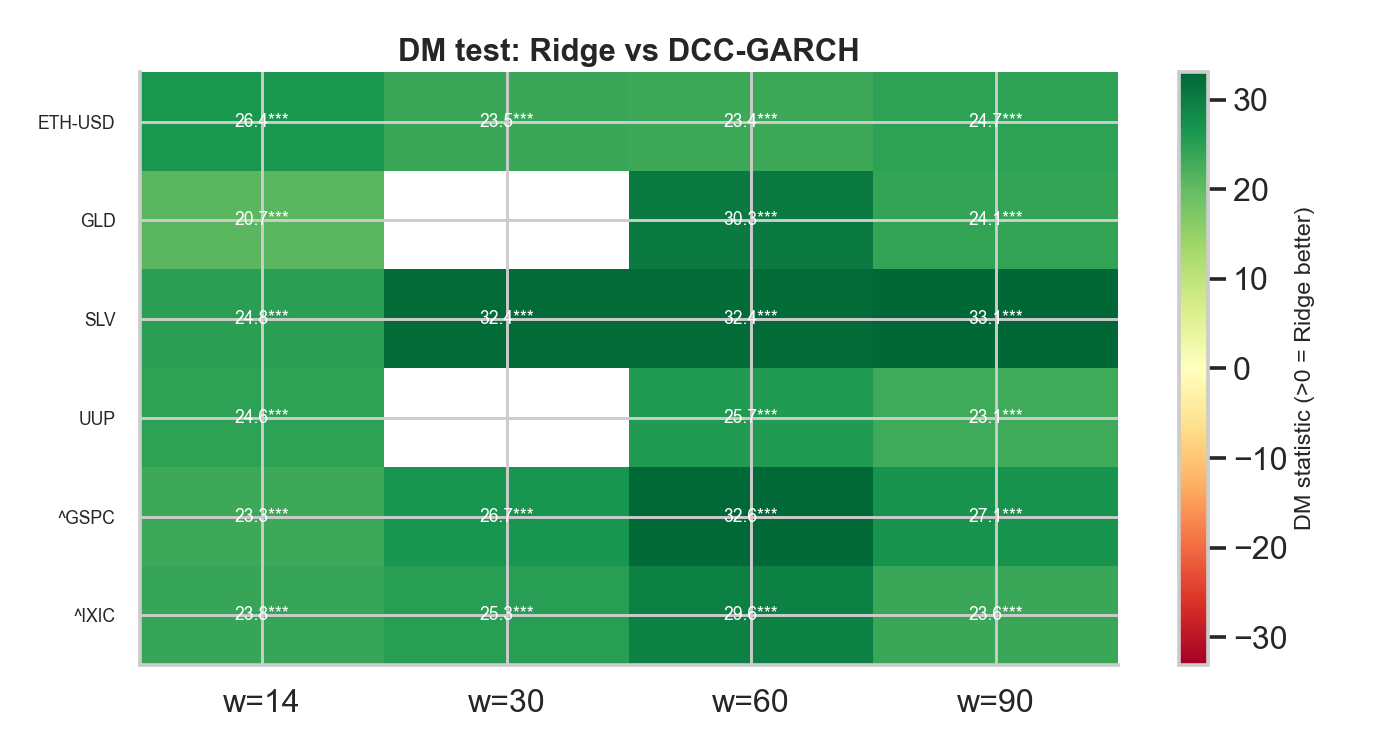
\includegraphics[width=0.82\textwidth]{../outputs/figures/dm_heatmap_Ridge_vs_DCC.png}
    \caption{Diebold--Mariano comparison against DCC-GARCH across dependency experiments.}
    \label{fig:dm_heatmap}
\end{figure}

The DM results support the claim that the strongest machine-learning model frequently outperforms DCC-GARCH in a statistically meaningful sense. This is an important result because it suggests that flexible predictive models can adapt more effectively than a classical conditional-correlation benchmark when the target is treated as a direct forecasting object.

At the same time, the DM analysis should not be overinterpreted. Beating DCC-GARCH does not imply beating persistence. The thesis therefore distinguishes clearly between \emph{benchmark superiority} and \emph{overall superiority}. Machine learning succeeds at the former more often than at the latter.

\subsection{Error-profile diagnostics}

Average error metrics summarize performance compactly, but they do not explain when models succeed or fail. The project therefore includes rolling RMSE diagnostics and forecast-error distribution plots. Figure~\ref{fig:rolling_rmse} illustrates how the error profile evolves through time for a representative experiment.

\begin{figure}[H]
    \centering
    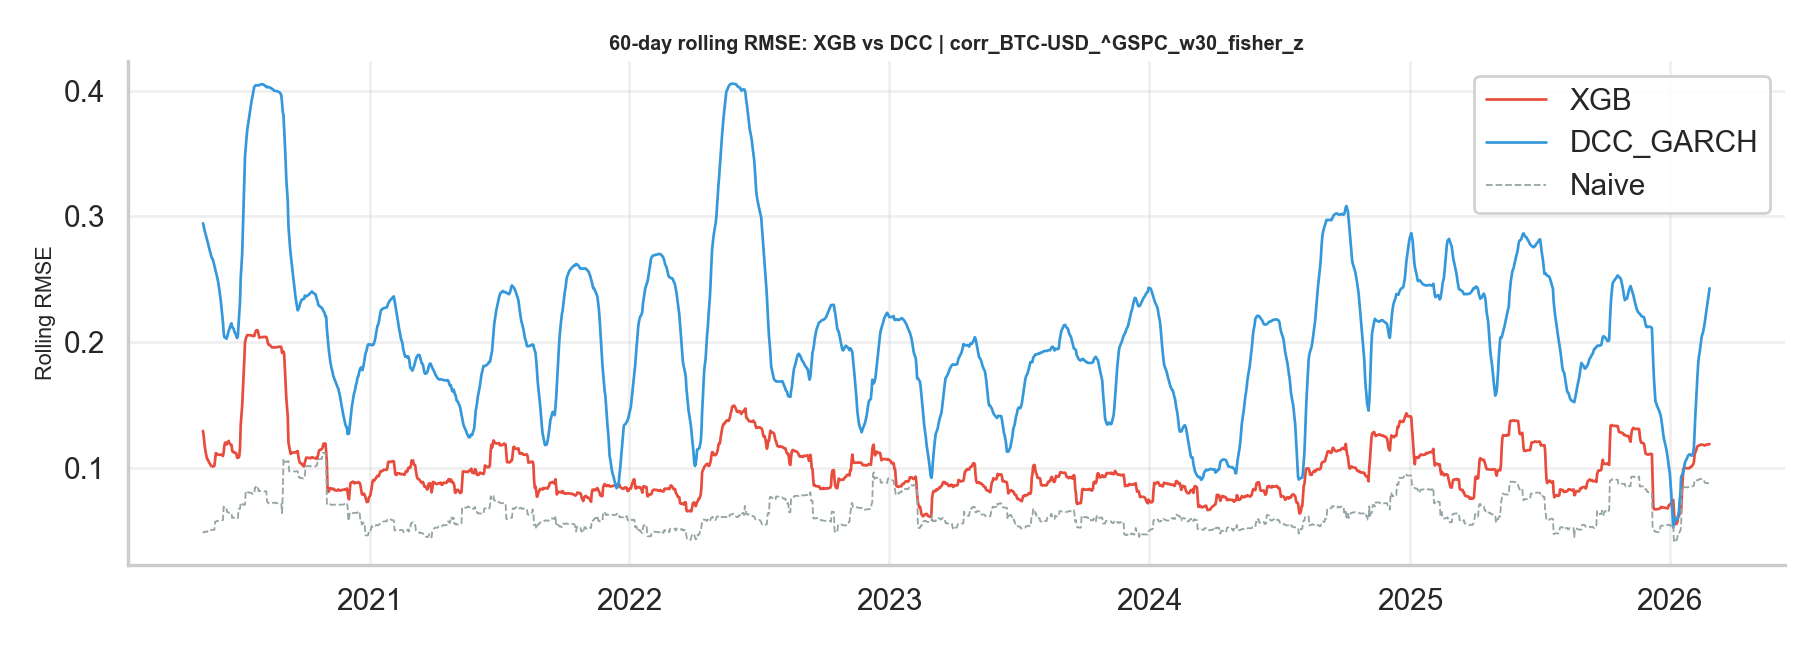
\includegraphics[width=0.9\textwidth]{../outputs/figures/rolling_rmse_corr_BTC-USD_^GSPC_w30_fisher_z.png}
    \caption{Rolling RMSE profile for the Bitcoin--S\&P 500 dependency forecast.}
    \label{fig:rolling_rmse}
\end{figure}

These diagnostics show that forecast quality is not constant through time. When the dependency process remains stable, even simple models perform well. When the market undergoes a regime transition, all models deteriorate, but the magnitude of the deterioration differs. This observation supports the practical value of model monitoring rather than one-off model selection.

The error-distribution and scatter diagnostics further show that the main challenge is not random noise alone but episodic underreaction to abrupt changes. In other words, the models tend to capture the low-frequency evolution of dependency better than the sharp turning points.

\subsection{Investor signal layer: average results}

The second empirical layer transforms crypto-derived information and dependency forecasts into a stress-warning problem. Table~\ref{tab:signal_summary} presents average classification results by model family.

\begin{table}[H]
    \centering
    \caption{Average investor-signal performance by classifier family.}
    \label{tab:signal_summary}
    \begin{tabular}{lrrr}
        \toprule
        Signal model & Balanced Accuracy & F1\_down & AUC \\
        \midrule
        Logit & 0.506 & 0.209 & 0.508 \\
        GBM\_Cls & 0.501 & 0.033 & 0.520 \\
        RF\_Cls & 0.500 & 0.030 & 0.519 \\
        \bottomrule
    \end{tabular}
\end{table}

The signal layer is deliberately more difficult than the first-layer regression problem. Stress-day detection is inherently noisy, class-imbalanced, and economically asymmetric. In this setting, the logistic model emerges as the most stable family. It does not produce spectacular scores, but it balances sensitivity and specificity better than the tree-based alternatives, which often collapse into extremely low exit rates and near-zero F1 for the downside class.

The correct interpretation is therefore moderate but positive. The signal layer is not strong enough to serve as a complete trading engine. However, it appears useful as a risk-management overlay, especially when applied to broad equity markets where avoiding a subset of stress periods may matter more than predicting every ordinary day.

\subsection{Best signal configurations}

The best single signal configurations occur for the S\&P 500 pair. In particular, the 30-day window combined with logistic classification reaches a Balanced Accuracy of 0.5405 and an F1 score of 0.2523 for the downside class. These values are not close to perfect prediction, but they are meaningfully above a purely random balanced baseline.

Figure~\ref{fig:signal_sp500} illustrates the signal output for the Bitcoin--S\&P 500 pair. The figure makes it easier to understand how the signal would be used in practice: not as a daily directional trade command, but as a warning indicator marking periods of elevated probability of stress.

\begin{figure}[H]
    \centering
    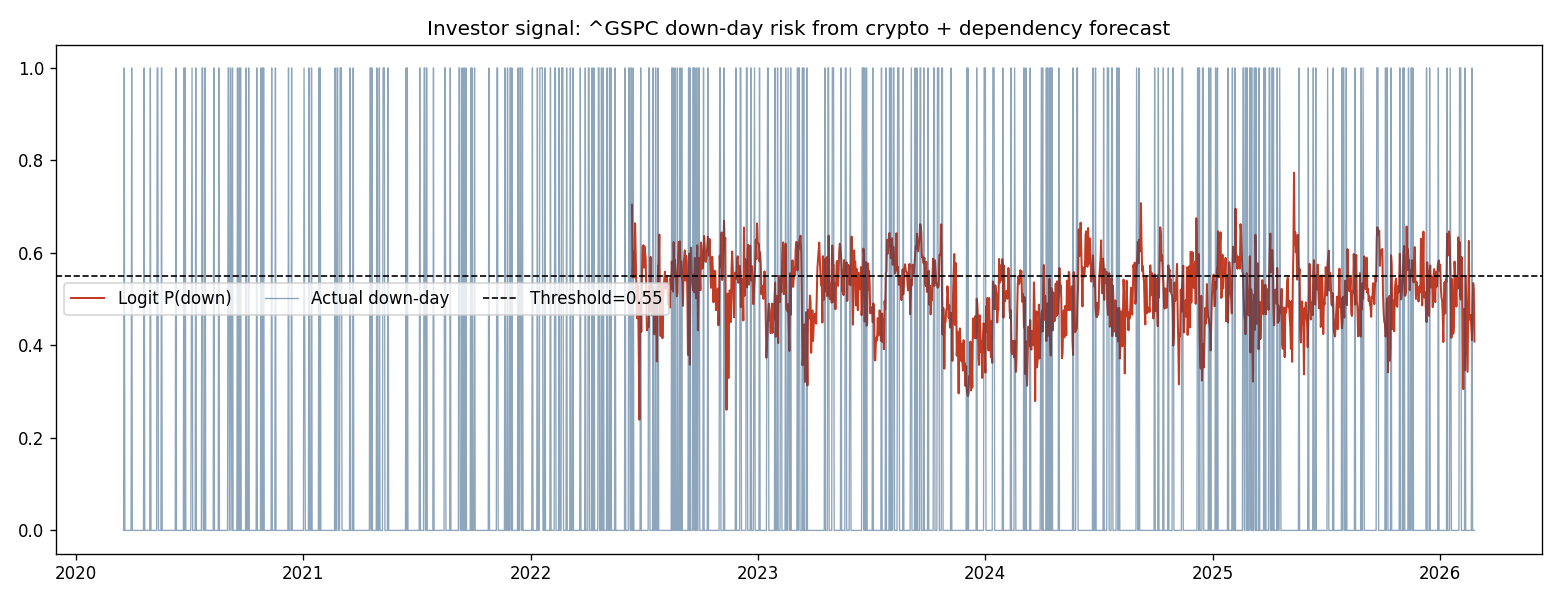
\includegraphics[width=0.95\textwidth]{../outputs/figures/signal_corr_BTC-USD_^GSPC_w30.png}
    \caption{Investor warning signal for stress days in the S\&P 500 market.}
    \label{fig:signal_sp500}
\end{figure}

For NASDAQ, metals, and the dollar proxy, the results are more mixed. This again suggests that the practical usefulness of the signal layer depends on market context. Equities appear more responsive to the kind of crypto-linked information captured by the feature set, whereas metal and currency proxies exhibit weaker and less stable signal behavior.

\subsection{Practical meaning of the signal layer}

A useful way to interpret the signal layer is through the question: what would a cautious investor do differently if the signal were available? The answer is not that the investor would trade every day. Rather, the signal would contribute to decisions about whether exposure should be reduced when market conditions become more fragile.

This practical framing aligns with the metrics reported in the project. Exit rate is an important complement to predictive accuracy because a model that almost never signals can look stable without being useful, while a model that signals too often may create excessive turnover. The logistic model occupies a middle ground that is more defensible from a portfolio-risk perspective.

\subsection{Sensitivity to window length}

Window length materially affects results. Short windows are more responsive but noisier; long windows are smoother but more inertial. This creates a trade-off between adaptability and stability. The experiments show that medium windows, especially 30 days, often provide a useful compromise. They preserve enough responsiveness to capture changing market structure while remaining smooth enough for stable one-step-ahead forecasting.

The sensitivity plots generated by the project also show that the apparent role of machine learning depends on this choice. With longer windows, persistence becomes even stronger and the relative advantage of complex models tends to diminish. This supports the broader thesis conclusion that the structure of the target itself largely determines the ranking of models.

\subsection{Summary of empirical findings}

The empirical results of the thesis can be summarized in four main statements:

\begin{enumerate}
    \item Time-varying dependency between Bitcoin and conventional assets is forecastable in an out-of-sample walk-forward setting.
    \item Most of the predictive power comes from persistence in the dependency process, which explains the strong performance of AR1 and naive baselines.
    \item Machine-learning models often outperform the DCC-GARCH benchmark, but usually do not outperform the strongest simple baselines on average.
    \item The investor signal layer delivers moderate, practically interpretable results and is best viewed as a risk-management aid rather than a standalone market-direction oracle.
\end{enumerate}

These results are coherent, internally consistent, and sufficient to support both the scientific and practical parts of the thesis. Their full interpretation is developed in the next section.
